%%%%%%%%%%%%%%%%%%%%%%%%%%%%%%%%%%%%%%%%%
% Beamer Presentation
% LaTeX Template
% Version 1.0 (10/11/12)
%
% This template has been downloaded from:
% http://www.LaTeXTemplates.com
%
% License:
% CC BY-NC-SA 3.0 (http://creativecommons.org/licenses/by-nc-sa/3.0/)
%
%%%%%%%%%%%%%%%%%%%%%%%%%%%%%%%%%%%%%%%%%

%----------------------------------------------------------------------------------------
%	PACKAGES AND THEMES
%----------------------------------------------------------------------------------------

\documentclass{beamer}

\mode<presentation> {

% The Beamer class comes with a number of default slide themes
% which change the colors and layouts of slides. Below this is a list
% of all the themes, uncomment each in turn to see what they look like.

%\usetheme{default}
%\usetheme{AnnArbor}
%\usetheme{Antibes}
%\usetheme{Bergen}
%\usetheme{Berkeley}
%\usetheme{Berlin}
%\usetheme{Boadilla}
%\usetheme{CambridgeUS}
%\usetheme{Copenhagen}
%\usetheme{Darmstadt}
%\usetheme{Dresden}
%\usetheme{Frankfurt}
%\usetheme{Goettingen}
%\usetheme{Hannover}
%\usetheme{Ilmenau}
%\usetheme{JuanLesPins}
%\usetheme{Luebeck}
\usetheme{Madrid}
%\usetheme{Malmoe}
%\usetheme{Marburg}
%\usetheme{Montpellier}
%\usetheme{PaloAlto}
%\usetheme{Pittsburgh}
%\usetheme{Rochester}
%\usetheme{Singapore}
%\usetheme{Szeged}
%\usetheme{Warsaw}

% As well as themes, the Beamer class has a number of color themes
% for any slide theme. Uncomment each of these in turn to see how it
% changes the colors of your current slide theme.

%\usecolortheme{albatross}
%\usecolortheme{beaver}
%\usecolortheme{beetle}
%\usecolortheme{crane}
%\usecolortheme{dolphin}
%\usecolortheme{dove}
%\usecolortheme{fly}
%\usecolortheme{lily}
%\usecolortheme{orchid}
%\usecolortheme{rose}
%\usecolortheme{seagull}
%\usecolortheme{seahorse}
%\usecolortheme{whale}
%\usecolortheme{wolverine}

%\setbeamertemplate{footline} % To remove the footer line in all slides uncomment this line
%\setbeamertemplate{footline}[page number] % To replace the footer line in all slides with a simple slide count uncomment this line

%\setbeamertemplate{navigation symbols}{} % To remove the navigation symbols from the bottom of all slides uncomment this line
}

\usepackage{graphicx} % Allows including images
\usepackage{booktabs} % Allows the use of \toprule, \midrule and \bottomrule in tables
\usepackage{verbatim}
\usepackage{datetime}
\usepackage{amsmath}
\usepackage{hyperref}
\usepackage{subfigmat}
\usepackage{epstopdf}
\usepackage{multicol}
\usepackage{tikz}
\usetikzlibrary{shapes,arrows}

\usepackage{tabularx} % for 'tabularx' environment
\usepackage{ragged2e} % for \Centering macro

\patchcmd{\subfigmatrix}{\hfill}{\hspace{0.8cm}}{}{}

\newcommand{\indentitem}{\setlength\itemindent{25pt}}
\newcommand{\tabitem}{~~\llap{\textbullet}~~}

%-----------------------------------------------------------------
% fixes the notes page item margin overflow

\tikzstyle{block} = [draw, fill=blue!20, rectangle, 
    minimum height=3em, minimum width=6em]
\tikzstyle{sum} = [draw, fill=blue!20, circle, node distance=1cm]
\tikzstyle{input} = [coordinate]
\tikzstyle{output} = [coordinate]
\tikzstyle{pinstyle} = [pin edge={to-,thin,black}]

\makeatletter
\defbeamertemplate{note page}{infolines}
{%
  {%
    \scriptsize
    \insertvrule{.25\paperheight}{white!90!black}
    \vskip-.25\paperheight
    \nointerlineskip
    \vbox{
      \hfill\insertslideintonotes{0.25}\hskip-\Gm@rmargin\hskip0pt%
      \vskip-0.25\paperheight%
      \nointerlineskip
      \begin{pgfpicture}{0cm}{0cm}{0cm}{0cm}
        \begin{pgflowlevelscope}{\pgftransformrotate{90}}
          {\pgftransformshift{\pgfpoint{-2cm}{0.2cm}}%
          \pgftext[base,left]{\footnotesize\the\year-\ifnum\month<10\relax0\fi\the\month-\ifnum\day<10\relax0\fi\the\day}}
        \end{pgflowlevelscope}
      \end{pgfpicture}}
    \nointerlineskip
    \vbox to .25\paperheight{\vskip0.5em
      \hbox{\insertshorttitle[width=8cm]}%
      \setbox\beamer@tempbox=\hbox{\insertsection}%
      \hbox{\ifdim\wd\beamer@tempbox>1pt{\hskip4pt\raise3pt\hbox{\vrule
            width0.4pt height7pt\vrule width 9pt
            height0.4pt}}\hskip1pt\hbox{\begin{minipage}[t]{7.5cm}\def\breakhere{}\insertsection\end{minipage}}\fi%
      }%
      \setbox\beamer@tempbox=\hbox{\insertsubsection}%
      \hbox{\ifdim\wd\beamer@tempbox>1pt{\hskip17.4pt\raise3pt\hbox{\vrule
            width0.4pt height7pt\vrule width 9pt
            height0.4pt}}\hskip1pt\hbox{\begin{minipage}[t]{7.5cm}\def\breakhere{}\insertsubsection\end{minipage}}\fi%
      }%
      \setbox\beamer@tempbox=\hbox{\insertshortframetitle}%
      \hbox{\ifdim\wd\beamer@tempbox>1pt{\hskip30.8pt\raise3pt\hbox{\vrule
            width0.4pt height7pt\vrule width 9pt
            height0.4pt}}\hskip1pt\hbox{\insertshortframetitle[width=7cm]}\fi%
      }%
      \vfil}%
  }%
\vskip.25em
\nointerlineskip
\begin{minipage}{\textwidth} % this is an addition
\insertnote
\end{minipage}               % this is an addition
}
\makeatother

\setbeamertemplate{note page}[infolines]
%-----------------------------------------------------------------

%\setbeameroption{show only notes}% un-comment to see the notes
%\setbeamertemplate{note page}[plain]

%\setbeamertemplate{itemize/enumerate body begin}{\normalsize}
\setbeamertemplate{itemize/enumerate subbody begin}{\footnotesize}

%\setbeamertemplate{caption}{\raggedright\insertcaption\par}

\setbeamerfont{caption}{size=\scriptsize}

\newcolumntype{C}{>{\Centering\arraybackslash}X}
\newcolumntype{L}{>{\raggedright\arraybackslash}X}

%----------------------------------------------------------------------------------------
%	TITLE PAGE
%----------------------------------------------------------------------------------------

\title[Mobile Biometrics - Face Recognition]{Mobile Biometrics - Face Recognition} % The short title appears at
% the bottom of every slide, the full title is only on the title page

\author{Adam Bronstein, Chris Brooks, Enrique Marquez} % Your name
\institute[ECS] % Your institution as it will appear on
% the bottom of every slide, may be shorthand to save space
{
University of Southampton \\ % Your institution for the title page
\medskip
\textit{arb2g11@soton.ac.uk, cjb1g14@soton.ac.uk, esm1g14@ecs.soton.ac.uk} % Your email address
}
\newdate{date}{12}{05}{2015}
\date{\displaydate{date}}
%\date{\today} % Date, can be changed to a custom date

\begin{document}

\begin{frame}
\titlepage % Print the title page as the first slide
\end{frame}

\begin{frame}
\frametitle{Contents} % Table of contents slide, comment this block out to remove it
\begin{columns}[t]
        \begin{column}{.5\textwidth}
            \tableofcontents[sections={1-4}]
        \end{column}
        \begin{column}{.5\textwidth}
            \tableofcontents[sections={5-8}]
        \end{column}
    \end{columns} % Throughout your presentation, if you choose to use \section{} and \subsection{} commands, these will automatically be printed on this slide as an overview of your presentation
\end{frame}

%----------------------------------------------------------------------------------------
%	PRESENTATION SLIDES
%----------------------------------------------------------------------------------------

%------------------------------------------------

\section{Face Recognition Overview} % A subsection can be created just before a set of
% slides with a common theme to further break down your presentation into chunks

%------------------------------------------------

\subsection{Issues}

\begin{frame}
\frametitle{Issues}

\begin{itemize}
  \item Checking the image contains a face
  \begin{itemize}
  	\item Lighting, scale and rotation invariant
  \end{itemize}
  \note{} 
  \item Using the correct internal representation
  \begin{itemize}
  	\item Need to be able to compare them
  	\item Small changes should have little effect
  \end{itemize}
  \note{} 
  \item Matching the faces correctly 
  \begin{itemize}
  	\item Need to be able to compare them
  \end{itemize}
\end{itemize}

\end{frame}

%------------------------------------------------

\subsection{Algorithm}

\begin{frame}[fragile] % Need to use the fragile option when verbatim is used in the slide
\frametitle{Face Recognition Algorithm}
% The block diagram code is probably more verbose than necessary
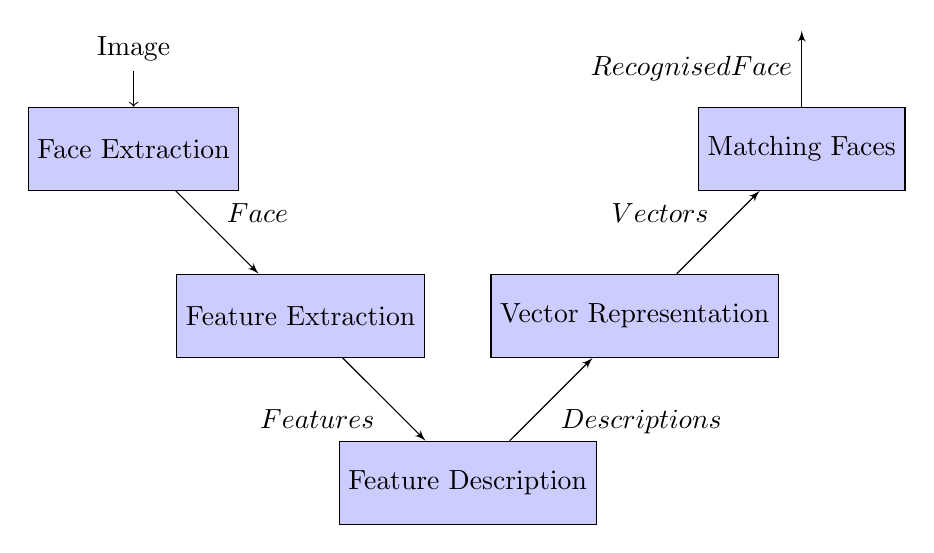
\begin{tikzpicture}[auto, node distance=2cm,>=latex']
    % We start by placing the blocks
    \node [block, name=face, pin={[pinstyle]above:Image}] {Face Extraction};
    \node [block, below right of=face, node distance=3cm] (feature) {Feature Extraction};
    \node [block, below right of=feature, node distance=3cm] (desc) {Feature Description};
    \node [block, above right of=desc, node distance=3cm] (vector) {Vector Representation};
    \node [block, above right of=vector, node distance=3cm] (matching) {Matching Faces};
    \node [output, above of=matching, node distance=1.5cm] (output) {};
    % We draw an edge between the face and feature block  
    \draw [->] (face) -- node[name=u] {$Face$} (feature);
    \draw [<-] (desc) -- node[name=v] {$Features$} (feature);
    \draw [<-] (vector) -- node[name=w] {$Descriptions$} (desc);
    \draw [->] (vector) -- node[name=x] {$Vectors$} (matching);
    \draw [->] (matching) -- node[name=y] {$Recognised Face$} (output);
\end{tikzpicture}
\end{frame}

%------------------------------------------------

\section{Face Extraction}

\subsection{Viola-Jones}

\begin{frame}
\frametitle{Viola-Jones}
\begin{columns}[c] % The "c" option specifies centered vertical alignment while the "t" option is used for top vertical alignment

\column{.5\textwidth} % Left column and width
\begin{itemize}
  \item Used to separate the face from the background
  \item Uses a trained Haar feature cascade classifier
  \item Detects all the faces in the picture
  \item Fast and lighting invariant 
  \item Not rotational invariant 
  \note{} 
\end{itemize}

\column{.5\textwidth} % Middle column and width
\begin{figure}[!htbp]
\centering
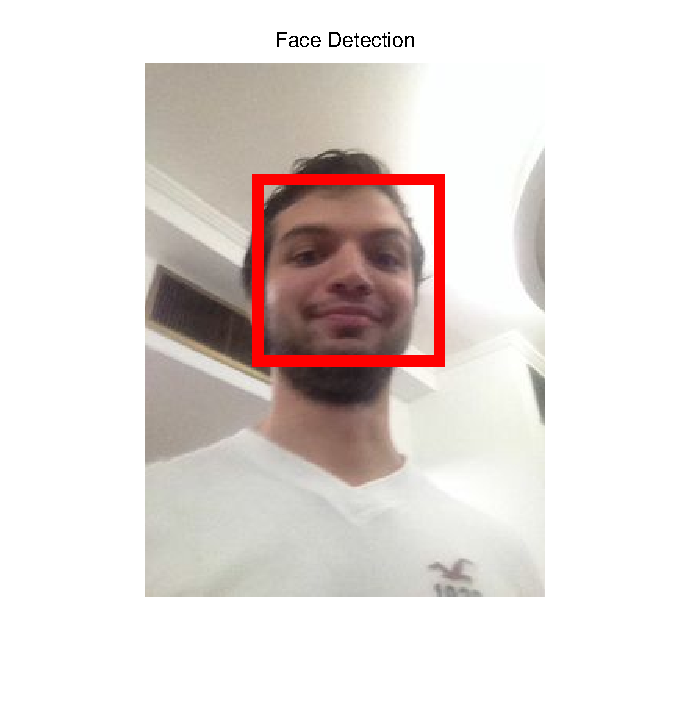
\includegraphics [totalheight=0.5\textheight] {Figures/ViolaJones.eps}
\caption{Face Detection with Viola-Jones}\label{fig:violajones}
\end{figure}

\end{columns}
\end{frame}

%------------------------------------------------

\section{Feature Extraction}

\subsection{Dense vs Interest Points}

\begin{frame}
\frametitle{Dense vs Interest Points}
\begin{columns}[c] % The "c" option specifies centered vertical alignment while the "t" option is used for top vertical alignment

\column{.5\textwidth} % Left column and width

\begin{itemize}
  \item Samples a grid around every pixel as a feature
  \item More points so it's robust, however this also makes it slow
  \note{} 
\end{itemize}


\column{.5\textwidth} % Middle column and width

\begin{itemize}
  \item Samples on interest point calculated by Harris corner detector or SIFT detector
  \item Fast, but might take into account too many irrelevant points 
  \note{} 
\end{itemize}

\end{columns}
\vspace{-10pt}
\begin{columns}[c] % The "c" option specifies centered vertical alignment while the "t" option is used for top vertical alignment

\column{.5\textwidth} % Left column and width

\begin{figure}[!htbp]
\centering
\includegraphics [totalheight=0.4\textheight] {Figures/dense.eps}
\vspace{-15pt}\caption{Dense Features}\label{fig:dense}
\end{figure}

\column{.5\textwidth} % Middle column and width

\begin{figure}[!htbp]
\centering
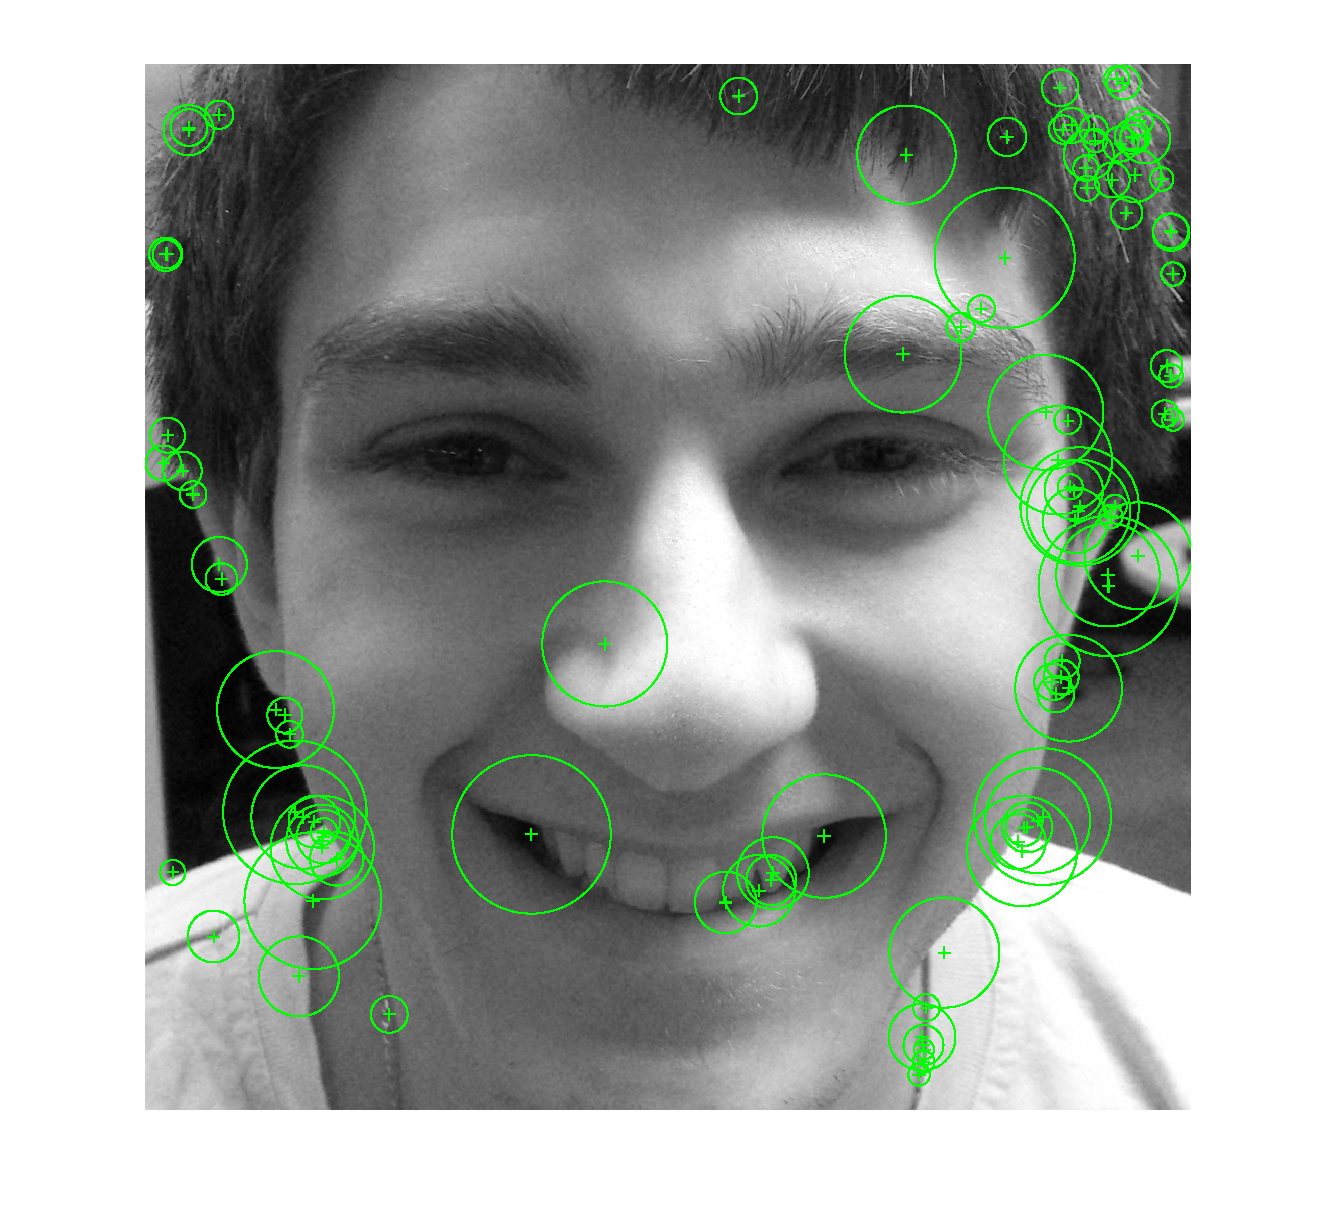
\includegraphics [totalheight=0.4\textheight] {Figures/featuresDetector.eps}
\vspace{-15pt}\caption{Interest Points}\label{fig:interest}
\end{figure}

\end{columns}

\end{frame}

%------------------------------------------------

\section{Feature Description}

\subsection{SIFT vs ORB}

\begin{frame}
\frametitle{SIFT vs ORB}

\begin{columns}[c] % The "c" option specifies centered vertical alignment while the "t" option is used for top vertical alignment

\column{1\textwidth} % Left column and width

\begin{itemize}
  \item SIFT has 128 Dimensions while ORB is only 32
  \item Similar accuracy 
  \note{} 
\end{itemize}

\end{columns}

\begin{columns}[c] % The "c" option specifies centered vertical alignment while the "t" option is used for top vertical alignment
\hspace{-50pt}
\column{.5\textwidth} % Left column and width
\begin{figure}[!htbp]
\centering
\includegraphics [totalheight=0.3\textheight] {Figures/phow_descriptors.eps}
\caption{SIFT Features}\label{fig:sift}
\end{figure}

\column{.5\textwidth} % Middle column and width
\begin{figure}[!htbp]
\centering
\includegraphics [totalheight=0.35\textheight] {Figures/orb_desriptors_sameperson.eps}
\caption{ORB Features}\label{fig:orb}
\end{figure}

\end{columns}
\end{frame}


\addtocontents{toc}{\newpage}

%------------------------------------------------

\section{Vector Representation}

\subsection{Bag of Visual Words (BoVW)}

\begin{frame}
\frametitle{Bag of Visual Words (BoVW)}
\begin{columns}[c] % The "c" option specifies centered vertical alignment while the "t" option is used for top vertical alignment

\column{.3\textwidth} % Left column and width

\column{.7\textwidth} % Middle column and width
{\fontsize{9}{11}\selectfont \hspace{18 mm} Training \hspace{4 mm} Matching \hspace{5 mm} Test}\\
{\fontsize{9}{11}\selectfont \hspace{22 mm} set \hspace{10 mm} norm \hspace{8 mm} image}
\end{columns}

\begin{columns}[c] % The "c" option specifies centered vertical alignment while the "t" option is used for top vertical alignment

\column{.3\textwidth} % Left column and width
\begin{itemize}
  \item Dense Sampling
  \item K-means 
  \item Database Representation
  \item Test Image Histogram Representation
  \item Matching (KNN)
  \note{} 
\end{itemize}

\column{.7\textwidth} % Middle column and width

\begin{figure}[!htbp]
\centering
\includegraphics [totalheight=0.5\textheight] {Figures/vbow_histogram.png}
\caption{Bag of Visual Words Histogram Matching}\label{fig:bovw}
\end{figure}

\end{columns}
\end{frame}

%------------------------------------------------

\subsection{Fisher Vectors}

\begin{frame}
\frametitle{Fisher Vectors}
\begin{columns}[c] % The "c" option specifies centered vertical alignment while the "t" option is used for top vertical alignment

\column{1\textwidth} % Left column and width
\begin{itemize}
  \item Takes BoVW one step further 
  \note{} 
\end{itemize}

\end{columns}
\begin{columns}[c] % The "c" option specifies centered vertical alignment while the "t" option is used for top vertical alignment

\column{1\textwidth} % Left column and width
\begin{figure}
\centering
\begin{tikzpicture}
\node[inner sep=0pt] (dense) 
    {\includegraphics[totalheight=0.25\textheight] {Figures/Dense.eps}};
\node[inner sep=0pt, below right of=dense, node distance=3cm] (gmm)
    {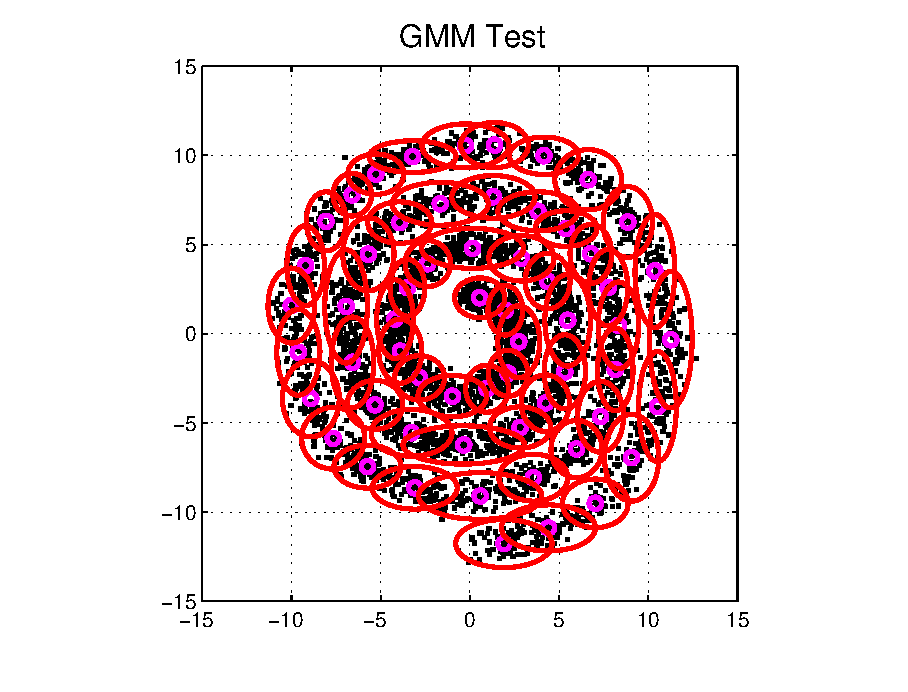
\includegraphics[totalheight=0.25\textheight] {Figures/GMM.eps}};
\node [block, right of=gmm, node distance=4cm, align=left] (equations) {\tiny $\Phi_{k}^{(1)} = \frac{1}{N\sqrt{w_k}}\Sigma_{p}^N \alpha_{p}(k)\Big(\frac{x_p-\mu_k}{\sigma_k}\Big)$ \\ \tiny $\Phi_{k}^{(2)} = \frac{1}{N\sqrt{2w_k}}\Sigma_{p}^N \alpha_{p}(k)\Big(\frac{(x_p-\mu_k)^2}{\sigma_{k}^{2}}-1\Big)$};
\node[inner sep=0pt, above right of=equations, node distance=3cm] (histogram)
    {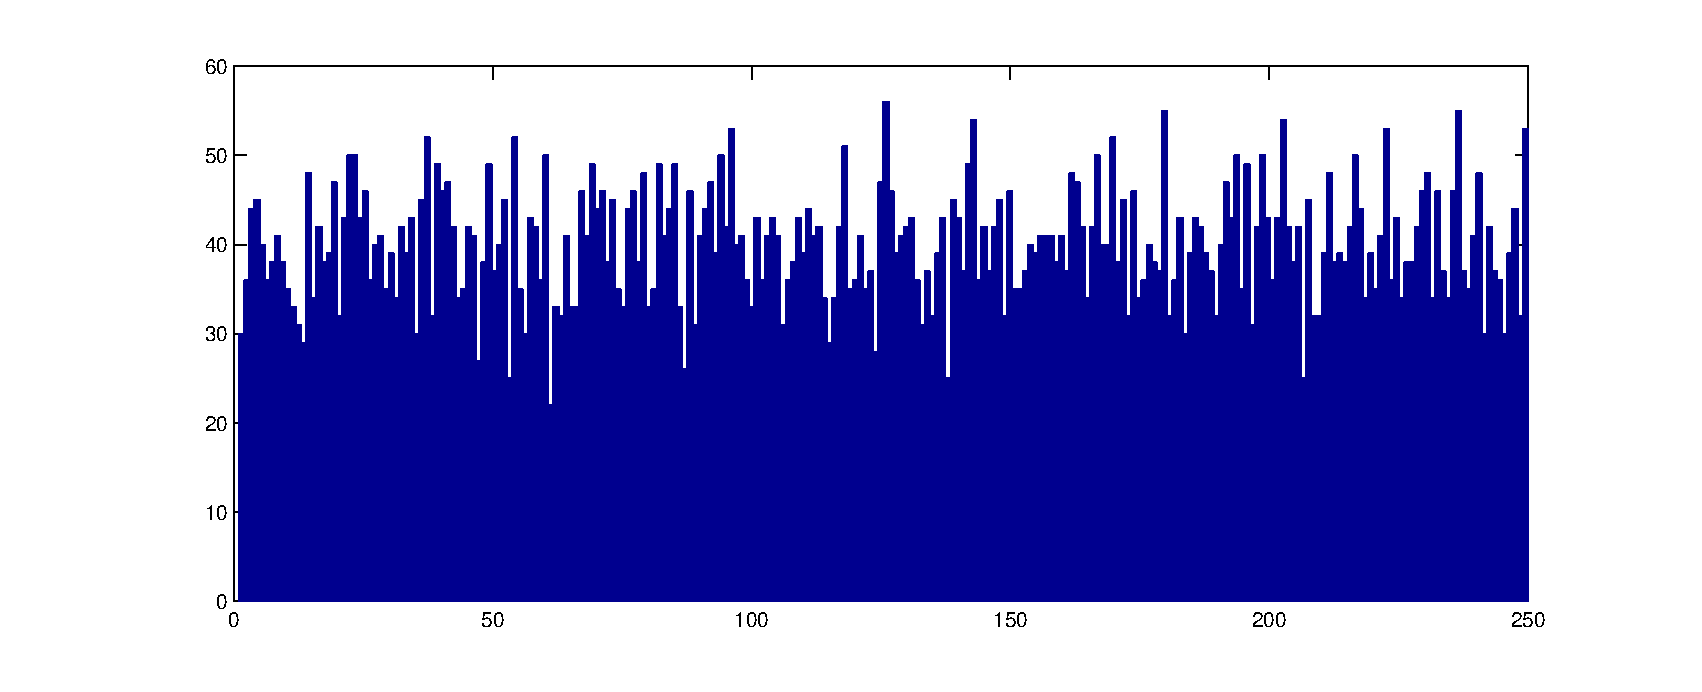
\includegraphics[totalheight=0.2\textheight] {Figures/hist.eps}};
\node [output, above of=histogram, node distance=2cm] (output) {};
\draw[<-,thick] (dense) -- (gmm);
\draw[->,thick] (gmm) -- (equations);
\draw[<-,thick] (histogram) -- (equations);
\draw [draw=white] (histogram) -- node[name=y] {$"Compact" Representation$} (output);
\end{tikzpicture}
\vspace{-15pt}\caption{Fisher Vector Process} \label{fig:fisher}
\end{figure}
\end{columns}

\end{frame}

%------------------------------------------------

\section{Mobile Face Recognition}

%------------------------------------------------

\subsection{Mobile Specific Issues}

\begin{frame}
\frametitle{Mobile Specific Issues}

\begin{itemize}
  \item Camera resolution
  \begin{itemize}
  	\item Two cameras, one worse than the other
  \end{itemize}
  \item Phone orientation
  \begin{itemize}
  	\item The phone can be held in many different orientations
  	\item It can also take the picture at different angles
  \end{itemize}
   \item Limited computing power
  \begin{itemize}
  	\item The memory is limited
  	\item Processor can be slow
  \end{itemize}
  \item Sift patented
  \begin{itemize}
  	\item Made it difficult to implement on opencv for Android
  \end{itemize}
  \note{} 
\end{itemize}

\end{frame}

%------------------------------------------------

\begin{frame}[fragile] % Need to use the fragile option when verbatim is used in the slide
\frametitle{Face Recognition Algorithm}
% The block diagram code is probably more verbose than necessary
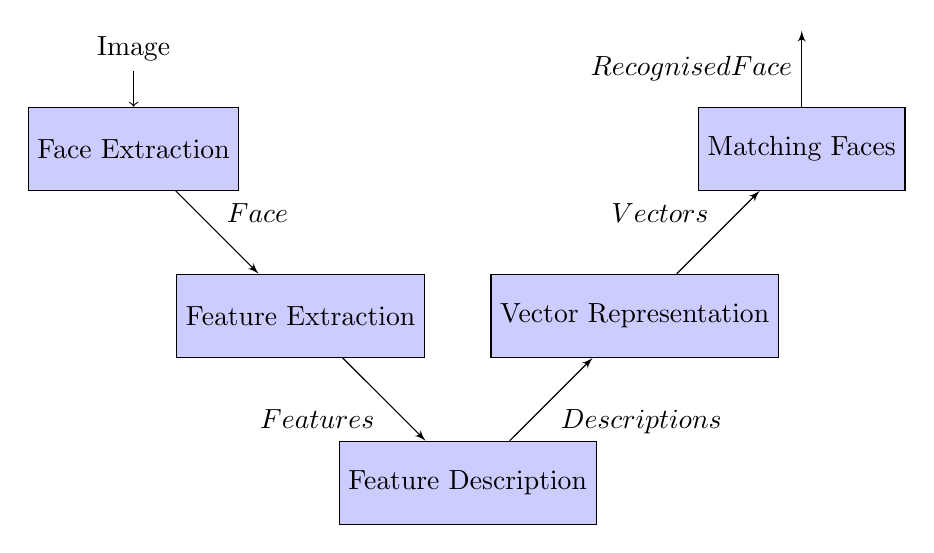
\begin{tikzpicture}[auto, node distance=2cm,>=latex']
    % We start by placing the blocks
    \node [block, name=face, pin={[pinstyle]above:Image}] {Face Extraction};
    \node [block, below right of=face, node distance=3cm] (feature) {Feature Extraction};
    \node [block, below right of=feature, node distance=3cm] (desc) {Feature Description};
    \node [block, above right of=desc, node distance=3cm] (vector) {Vector Representation};
    \node [block, above right of=vector, node distance=3cm] (matching) {Matching Faces};
    \node [output, above of=matching, node distance=1.5cm] (output) {};
    % We draw an edge between the face and feature block  
    \draw [->] (face) -- node[name=u] {$Face$} (feature);
    \draw [<-] (desc) -- node[name=v] {$Features$} (feature);
    \draw [<-] (vector) -- node[name=w] {$Descriptions$} (desc);
    \draw [->] (vector) -- node[name=x] {$Vectors$} (matching);
    \draw [->] (matching) -- node[name=y] {$Recognised Face$} (output);
\end{tikzpicture}
\end{frame}

%------------------------------------------------

\subsection{Algorithms}

\begin{frame}[fragile] % Need to use the fragile option when verbatim is used in the slide
\frametitle{First Face Recognition Algorithm}
% The block diagram code is probably more verbose than necessary
\begin{tikzpicture}[auto, node distance=2cm,>=latex']
    % We start by placing the blocks
    \node [block, name=face, pin={[pinstyle]above:Image}] {Viola-Jones};
    \node [block, below right of=face, node distance=3cm] (feature) {Interest points};
    \node [block, below right of=feature, node distance=3cm] (desc) {ORB};
    \node [block, above right of=vector, node distance=3cm] (matching) {KNN};
    \node [output, above of=matching, node distance=1.5cm] (output) {};
    % We draw an edge between the face and feature block  
    \draw [->] (face) -- node[name=u] {$Face$} (feature);
    \draw [<-] (desc) -- node[name=v] {$Features$} (feature);
    \draw [<-] (matching) -- node[name=w] {$Descriptions$} (desc);
    \draw [->] (matching) -- node[name=y] {$Recognised Face$} (output);
\end{tikzpicture}
\end{frame}

%------------------------------------------------

\begin{frame}[fragile] % Need to use the fragile option when verbatim is used in the slide
\frametitle{Second Face Recognition Algorithm}
% The block diagram code is probably more verbose than necessary
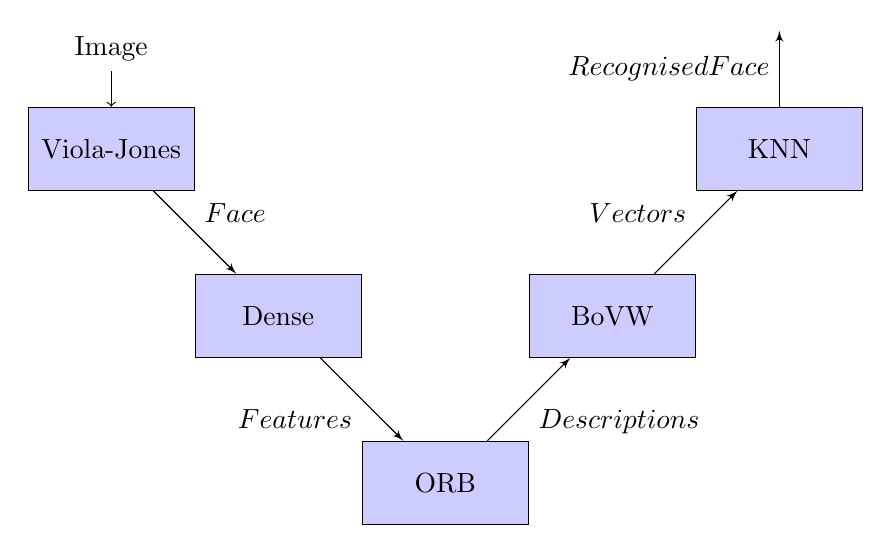
\begin{tikzpicture}[auto, node distance=2cm,>=latex']
    % We start by placing the blocks
    \node [block, name=face, pin={[pinstyle]above:Image}] {Viola-Jones};
    \node [block, below right of=face, node distance=3cm] (feature) {Dense};
    \node [block, below right of=feature, node distance=3cm] (desc) {ORB};
    \node [block, above right of=desc, node distance=3cm] (vector) {BoVW};
    \node [block, above right of=vector, node distance=3cm] (matching) {KNN};
    \node [output, above of=matching, node distance=1.5cm] (output) {};
    % We draw an edge between the face and feature block  
    \draw [->] (face) -- node[name=u] {$Face$} (feature);
    \draw [<-] (desc) -- node[name=v] {$Features$} (feature);
    \draw [<-] (vector) -- node[name=w] {$Descriptions$} (desc);
    \draw [->] (vector) -- node[name=x] {$Vectors$} (matching);
    \draw [->] (matching) -- node[name=y] {$Recognised Face$} (output);
\end{tikzpicture}
\end{frame}

%------------------------------------------------

\begin{frame}[fragile] % Need to use the fragile option when verbatim is used in the slide
\frametitle{Third Face Recognition Algorithm}
% The block diagram code is probably more verbose than necessary
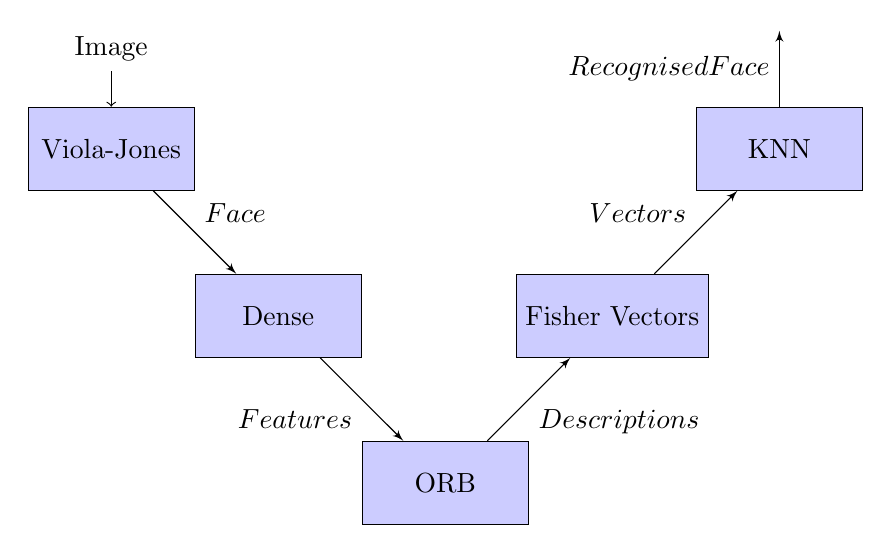
\begin{tikzpicture}[auto, node distance=2cm,>=latex']
    % We start by placing the blocks
    \node [block, name=face, pin={[pinstyle]above:Image}] {Viola-Jones};
    \node [block, below right of=face, node distance=3cm] (feature) {Dense};
    \node [block, below right of=feature, node distance=3cm] (desc) {ORB};
    \node [block, above right of=desc, node distance=3cm] (vector) {Fisher Vectors};
    \node [block, above right of=vector, node distance=3cm] (matching) {KNN};
    \node [output, above of=matching, node distance=1.5cm] (output) {};
    % We draw an edge between the face and feature block  
    \draw [->] (face) -- node[name=u] {$Face$} (feature);
    \draw [<-] (desc) -- node[name=v] {$Features$} (feature);
    \draw [<-] (vector) -- node[name=w] {$Descriptions$} (desc);
    \draw [->] (vector) -- node[name=x] {$Vectors$} (matching);
    \draw [->] (matching) -- node[name=y] {$Recognised Face$} (output);
\end{tikzpicture}
\end{frame}

%------------------------------------------------

\subsection{Algorithm Comparison}

\begin{frame}
\frametitle{Algorithm Comparison}
\begin{table}
\begin{tabular}{l l l l}
\toprule
\textbf{Training dataset size} & \textbf{Fisher Vectors} & \textbf{BoVW}\\
\midrule
20\% & 91.25\% & 69.7\% \\
50\% & 98.50\% & 77\% \\
80\% &100\% & 86.25\% \\
\bottomrule
\end{tabular}
\caption{Compares accuracy of methods as training set size increases using AT\&T Faces Dataset}
\end{table}
\end{frame}

%------------------------------------------------

\section{Demo}

%------------------------------------------------

\subsection{Add Person}

\begin{frame}
\frametitle{Add Person}
\begin{columns}[c] % The "c" option specifies centered vertical alignment while the "t" option is used for top vertical alignment

\column{.3\textwidth} % Left column and width
\begin{figure}[!htbp]
\centering
\includegraphics [totalheight=0.65\textheight] {Figures/mainscreen.png}
\caption{Main Screen}\label{fig:main1}
\end{figure}

\column{.3\textwidth} % Middle column and width
\begin{figure}[!htbp]
\centering
\includegraphics [totalheight=0.65\textheight] {Figures/takepicture.png}
\caption{Take Picture}\label{fig:take1}
\end{figure}

\column{.3\textwidth} % Right column and width
\begin{figure}[!htbp]
\centering
\includegraphics [totalheight=0.65\textheight] {Figures/addperson.png}
\caption{Add Person}\label{fig:add}
\end{figure}

\end{columns}
\end{frame}

%------------------------------------------------

\subsection{Recognise Person}

\begin{frame}
\frametitle{Recognise Person}
\begin{columns}[c] % The "c" option specifies centered vertical alignment while the "t" option is used for top vertical alignment

\column{.3\textwidth} % Left column and width
\begin{figure}[!htbp]
\centering
\includegraphics [totalheight=0.65\textheight] {Figures/mainscreen.png}
\caption{Main Screen}\label{fig:main2}
\end{figure}

\column{.3\textwidth} % Middle column and width
\begin{figure}[!htbp]
\centering
\includegraphics [totalheight=0.65\textheight] {Figures/takepicture.png}
\caption{Take Picture}\label{fig:take2}
\end{figure}

\column{.3\textwidth} % Right column and width
\begin{figure}[!htbp]
\centering
\includegraphics [totalheight=0.65\textheight] {Figures/recogniseperson.png}
\caption{Recognise Person}\label{fig:recognise}
\end{figure}

\end{columns}
\end{frame}

%------------------------------------------------

\begin{frame}
\Huge{\centerline{Any questions?}}
\end{frame}

%------------------------------------------------

\begin{frame}
\frametitle{References}
\footnotesize{
\begin{thebibliography}{99} % Beamer does not support BibTeX so references must be inserted manually as below
\bibitem[Perronnin, 2006]{p2} F. Perronnin and C. Dance. Fisher kernels on
visual vocabularies for image categorizaton. In Proc. CVPR, 2006.
\bibitem[Simonyan, 2013]{p3} Simonyan, K. and Parkhi, O. M. and Vedaldi, A. and
Zisserman, A. Fisher Vector Faces in the Wild. British Machine Vision
Conference, 2013.
\bibitem[Rublee, 2011]{p4} E. Rublee, V. Rabaud, K. Konolige, and G. Bradski.
ORB:
an efficient alternative to SIFT or SURF. In Proc. of the IEEE Intl. Conf. on Computer Vision (ICCV), volume 13, 2011.
\bibitem[Vedaldi, 2008]{p5} A. Vedaldi and B. Fulkerson VLFeat: An Open and
Portable Library of Computer Vision Algorithms, 2008. Available at:
\textless\url{http://www.vlfeat.org/}[Accessed 26th April 2015]
\bibitem[Bradski, 2000]{p6} G. Bradski The OpenCV Library. Dr. Dobb�s Journal
of Software Tools, 2000. \textless\url{http://www.opencv.org/}[Accessed 26th April
2015]
\end{thebibliography}
}
\end{frame}

%------------------------------------------------

\begin{comment}

%------------------------------------------------

\begin{frame}
\frametitle{Paragraphs of Text}
Sed iaculis dapibus gravida. Morbi sed tortor erat, nec interdum arcu. Sed id lorem lectus. Quisque viverra augue id sem ornare non aliquam nibh tristique. Aenean in ligula nisl. Nulla sed tellus ipsum. Donec vestibulum ligula non lorem vulputate fermentum accumsan neque mollis.\\~\\

Sed diam enim, sagittis nec condimentum sit amet, ullamcorper sit amet libero. Aliquam vel dui orci, a porta odio. Nullam id suscipit ipsum. Aenean lobortis commodo sem, ut commodo leo gravida vitae. Pellentesque vehicula ante iaculis arcu pretium rutrum eget sit amet purus. Integer ornare nulla quis neque ultrices lobortis. Vestibulum ultrices tincidunt libero, quis commodo erat ullamcorper id.
\end{frame}

%------------------------------------------------

\begin{frame}
\frametitle{Bullet Points}
\begin{itemize}
  \item Lorem ipsum dolor sit amet, consectetur adipiscing elit
  \item Aliquam blandit faucibus nisi, sit amet dapibus enim tempus eu
  \item Nulla commodo, erat quis gravida posuere, elit lacus lobortis est, quis porttitor odio mauris at libero
  \item Nam cursus est eget velit posuere pellentesque
  \item Vestibulum faucibus velit a augue condimentum quis convallis nulla gravida
\end{itemize}
\end{frame}

%------------------------------------------------

\begin{frame}
\frametitle{Blocks of Highlighted Text}% blue blocks
\begin{block}{Block 1}
Lorem ipsum dolor sit amet, consectetur adipiscing elit. Integer lectus nisl, ultricies in feugiat rutrum, porttitor sit amet augue. Aliquam ut tortor mauris. Sed volutpat ante purus, quis accumsan dolor.
\end{block}

\begin{block}{Block 2}
Pellentesque sed tellus purus. Class aptent taciti sociosqu ad litora torquent per conubia nostra, per inceptos himenaeos. Vestibulum quis magna at risus dictum tempor eu vitae velit.
\end{block}

\begin{block}{Block 3}
Suspendisse tincidunt sagittis gravida. Curabitur condimentum, enim sed venenatis rutrum, ipsum neque consectetur orci, sed blandit justo nisi ac lacus.
\end{block}
\end{frame}

%------------------------------------------------

\begin{frame}
\frametitle{Multiple Columns}
\begin{columns}[c] % The "c" option specifies centered vertical alignment while the "t" option is used for top vertical alignment

\column{.45\textwidth} % Left column and width
\textbf{Heading}
\begin{enumerate}
  \item Statement
  \item Explanation
  \item Example
\end{enumerate}

\column{.5\textwidth} % Right column and width
Lorem ipsum dolor sit amet, consectetur adipiscing elit. Integer lectus nisl, ultricies in feugiat rutrum, porttitor sit amet augue. Aliquam ut tortor mauris. Sed volutpat ante purus, quis accumsan dolor.

\end{columns}
\end{frame}

%------------------------------------------------
\section{Second Section}
%------------------------------------------------

\begin{frame}
\frametitle{Table}
\begin{table}
\begin{tabular}{l l l}
\toprule
\textbf{Treatments} & \textbf{Response 1} & \textbf{Response 2}\\
\midrule
Treatment 1 & 0.0003262 & 0.562 \\
Treatment 2 & 0.0015681 & 0.910 \\
Treatment 3 & 0.0009271 & 0.296 \\
\bottomrule
\end{tabular}
\caption{Table caption}
\end{table}
\end{frame}

%------------------------------------------------

\begin{frame}
\frametitle{Theorem}
\begin{theorem}[Mass--energy equivalence] %inside a blue block
$E = mc^2$
\end{theorem}
\end{frame}

%------------------------------------------------

\begin{frame}[fragile] % Need to use the fragile option when verbatim is used in the slide
\frametitle{Verbatim}
\begin{example}[Theorem Slide Code] % inside green block
\begin{verbatim}
\begin{frame}
\frametitle{Theorem}
\begin{theorem}[Mass--energy equivalence]
$E = mc^2$
\end{theorem}
\end{frame}\end{verbatim}
\end{example}
\end{frame}

%------------------------------------------------

\begin{frame}
\frametitle{Figure}
Uncomment the code on this slide to include your own image from the same directory as the template .TeX file.
%\begin{figure}
%\includegraphics[width=0.8\linewidth]{test}
%\end{figure}
\end{frame}

%------------------------------------------------

\begin{frame}[fragile] % Need to use the fragile option when verbatim is used in the slide
\frametitle{Citation}
An example of the \verb|\cite| command to cite within the presentation:\\~

This statement requires citation \cite{p1}.
\end{frame}

%------------------------------------------------

\begin{frame}
\frametitle{References}
\footnotesize{
\begin{thebibliography}{99} % Beamer does not support BibTeX so references must be inserted manually as below
\bibitem[Smith, 2012]{p1} John Smith (2012)
\newblock Title of the publication
\newblock \emph{Journal Name} 12(3), 45 -- 678.
\end{thebibliography}
}
\end{frame}

%------------------------------------------------

\begin{frame}
\Huge{\centerline{The End}}
\end{frame}

%----------------------------------------------------------------------------------------

\end{comment}

\end{document}